%!TEX root = ../marisa-thesis.tex

\chapter*{Notation}
$W_G^i(n)$ = the number of closed walks of length $n$ at vertex $i$\\
$W_G(n)$ = the number of closed walks of length $n$ for graph $G$ \\
$G_{i,j}$ = the molecular graph of $C_iH_j$
\chapter{Background Information}
\section{Linear Algebra}
Linear Algebra is the study of vectors and linear transformations. Transformations in this section will be matrices. A matrix is the result of organizing information related to linear transformations. Matrices of the same size can be added together and matrices that are not of the same size can be multiplied together.  Moreover, we can evaluate matrices when they are in ``reduced row echleon form.''
\par Throughout this research we use something called the determinant.  The determinant takes a square matrix (an $n\times n$ matrix) and makes it into a single number.  It is denoted as $\det(A)$ where A is the matrix.  If $\det(A)\neq0$ then the matrix is invertible.  For our purposes, we want the matrix to not equal zero.  To find the total number of closed walks within our graph we must be able to find the determinant of the eigenvalues.
\subsection{Linear Algebra Definitions}
There are many definitions that can give background to the research conducted when evaluating combinatorics and the different graphs studied.  There are many connections that mathematics contains for this field of work.  These parts of mathematics that help explain the work done includes: Linear Algebra, which is defined before, Graph Theory, and Combinatorics. Each field will contain different aspects that will be useful in the research done.  
\theoremstyle{definition}
\newtheorem{exmp}{Example}[section]
\begin{definition}[Linear Transformation]
Let $V, W$ be vector spaces over a field, $\mathbb{F}$. The map
    $$T: V \rightarrow W$$ is a linear transformation if $$T(\alpha v + \beta w) = \alpha Tv + \beta Tw.$$ For all $v, w \in V$ \& $\alpha, \beta \in \mathbb{F}$.
\end{definition}

\begin{exmp}
     Let the mapping $$T: \mathbb{R}^1 \rightarrow \mathbb{R}^1$$ be defined by \[ T(x)=3x. \]
\end{exmp}
\begin{figure}[h]
         \centering
         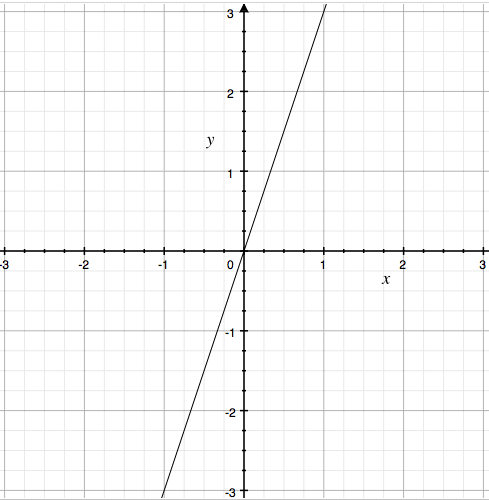
\includegraphics[width = 2.0in]{3x.png}
         \caption{\small{A graphical representation of $$T(x)= 3x$$}}
 \end{figure}
Let us evaluate the example: 

    \begin{align*}
    T(\alpha v + \beta w) = 3(\alpha v + \beta w).\\
    \alpha T(v) + \beta T(w) = 3v + \alpha 3v + \beta 3w = 3(\alpha v + \beta w).
    \end{align*} 

They are equal! It's worth noting that this example works for all lines through the origin. 
\begin{exmp}
We can also view $T$ as a matrix. Let the matrix $T$ have the mapping $$\mathbb{R}^2 \rightarrow \mathbb{R}^2$$ and be represented by:
\end{exmp}

$$
 \begin{bmatrix}
    
    1   &   2 \\
    0   &   4 \\
\end{bmatrix}
$$
where

 \[
 v = \begin{bmatrix}
       v_{1}\\
       v_{2}\\
      \end{bmatrix}
 \] 
 ,
 \[ w = \begin{bmatrix}
       w_{1}\\
       w_{2}\\
      \end{bmatrix}
 \]
 \[ \alpha, \beta \in \mathbb{R}\]
 \\
 \begin{align*}
 \begin{bmatrix}
    1   &   2 \\
    0   &   4 \\
\end{bmatrix}
\times \alpha \left(\begin{bmatrix}
       v_{1}\\
       v_{2}\\
      \end{bmatrix} \right)
    + \left(\beta \begin{bmatrix}
       w_{1}\\
       w_{2}\\
      \end{bmatrix}\right) = 
\begin{bmatrix}
    1   &   2 \\
    0   &   4 
\end{bmatrix}
\begin{bmatrix}
    \alpha(v_{1}) + \beta(w_{1}) \\
     \alpha(v_{2}) + \beta(w_{2}) \\
\end{bmatrix}
= \\
\begin{bmatrix}
    (\alpha(v_{1}) + \beta(w_{1})) + 2(\alpha(v_{2} + \beta(w_{2})) \\
    4(\alpha(v_{2} + \beta(W_{2})) \\
\end{bmatrix}
= \\
\alpha \left( 
\begin{bmatrix}
     1   &   2 \\
    0   &   4 \\
\end{bmatrix}\right)
\begin{bmatrix}
       v_{1}\\
       v_{2}\\
      \end{bmatrix}
+ 
\beta \left(
\begin{bmatrix}
     1   &   2 \\
    0   &   4 \\
\end{bmatrix} \right)
\begin{bmatrix}
       w_{1}\\
       w_{2}\\
      \end{bmatrix}\\
  \end{align*}

\begin{definition}[Determinant $2\times2$]
    The determinant of a $2 \times 2$ matrix is given by    
\end{definition}
 \[
     \det\begin{bmatrix}
         a & b \\
         c & d  \\ 
     \end{bmatrix} 
    = ad - cd. \]

\begin{exmp}
  Let us find the determinant of the matrix below: 

$$\det \begin{bmatrix}
       1 & 2 \\
       3 & 4  \\ 
    \end{bmatrix}
    = 4 - 6 = -2.$$
Here we performed the operation of multiplication with $1 \times 4$ and subtracted this answer with $2 \times 3$.  This resulted in the answer $-2$. Thus, the determinant of the matrix is $-2$. \\
\end{exmp}

We can generalize this to $n \times n$ matrices recursively. But we need certain tools first. \\
% source for transpose, minor and cofactor: https://www.math.ucdavis.edu/~linear/linear-guest.pdf
\begin{definition}[Minors]
    A minor of an $n\times n$ matrix $M$ is the determinant of any square matrix obtained from $M$ by deleting one row and one column. In other words, any entry $m^{i}_{j}$ of a square matrix $M$ is associated to a minor obtained by deleting the $i$th row and the $j$th column of $M$.  Minors are represented by $M_{i,j}$
\end{definition}
\begin{definition}[Cofactors]
    A cofactors is represented as $m_{i,j}$.  The cofactor of $M$ corresponding to the entry $m_{j}^{i}$ of $M$ is the product of the minor associated to $m_{j}^{i}$ and $(-1)^{i+j}$. 
\end{definition}

Therefore, we can evaluate matrices that are greater than $2 \times 2$.

\begin{definition}[Determinant of an $n \times n$]
    The determinant of an $n \times n$ matrix $M$ is shown by

   $$ \det(M) = \Sigma (c_{i,j} \times M_{i,j}) $$

\end{definition}
When evaluating the answer for the given matrix, the signs of the equation should be folliowed. These signs are represented from the matrix below.
\[
\begin{bmatrix}
    +  & - & + \\
    -  & + & - \\
    +  & - & \ddots \\
    
\end{bmatrix}
  \]  

\begin{definition}[Transpose]
    The transpose of a column vector is the corresponding row vector and vice versa:
\end{definition}
\begin{exmp}
  Let $v=$ \[ \begin{pmatrix}
        1 \\
        2  \\
        3
  \end{pmatrix}.\]
  Then
  $v^T =$
  \[
  \begin{pmatrix}
    1 \, 2 \, 3
  \end{pmatrix}\]
  and $(v^T)^T = v$  This is because an operation performed twice does not affect the equation. 
\end{exmp}
\begin{proposition}
  If $M$ is a square matrix then $\det M^T = \det M$
\end{proposition}
\begin{proof}
  We know that the determinant can be computed by a cofactor expansion along any row or column. \\

  Let us prove this by induction on $n$. For the base case $n=1$ we have $A = A^T$, thus 
  $$\det A = \det A^T$$.  This is what we wanted thus we can move to our inductive step. Let us assume the result is true for $n = k-1$ and let $A$ be a $k \times k$ matrix.
  Let the matrix $A =$
  \[
  \begin{bmatrix}
     a_{11}  &   a_{12}  &   \hdots  & a_{1k} \\
     a_{21}  &   a_{22}  &   \hdots  & a_{2k} \\
        \vdots  &   \vdots  & \ddots & \vdots \\
    a_{k1}       &   a_{k1}     &   \hdots  & a_{kk} \\
  \end{bmatrix}\] so that 
  $A^T =$
  \[
  \begin{bmatrix}
     a_{11}  &   a_{21}  &   \hdots  & a_{k1} \\
     a_{12}  &   a_{22}  &   \hdots  & a_{k2} \\
        \vdots  &   \vdots  & \ddots & \vdots \\
    a_{1k}       &   a_{2k}     &   \hdots  & a_{kk} \\
  \end{bmatrix}\]
  Using cofactor expansion along the first column of $A$ we have\\ $\det A = a_{11} \det A_{11}-a_{21} \det A_{21}+ ... +(-1)^{k+1}a_{k1}\det A_{k1}$, where $A_{i,j}$ is the matrix obtained from $A$ by removing the $i$th row and the $j$th column. Using cofactor expansion along the first row of $A^T$ we have: \\
  $\det (A^T) = a_{11} \det (A^T)_{11}-a_{21} \det (A^T)_{12}+ ... +(-1)^{k+1}a_{k1}\det (A^T)_{1k}$ \\\\
  We notice that $(A^T)_{ij}=(A_{ij})^T$. Since $A_{ji}$ is a $(k-1) \times (k-1)$ matrix we can use the inductive hypothesis to see that\\
  $\det (A^T)_{ij} = \det((A_{ij}^T)= \det A_{ij}.$ \\

  If we subsitute this to the above formula for $\det(A^T)$ we get \\
  $\det(A^T)= \det A$. \\
\end{proof}
There are some properties that we should consider that involve elementary row operations and determinants. 
 % source textbook: https://www.math.purdue.edu/files/academic/courses/2010spring/MA26200/3_2.pdf\\
\begin{enumerate}
    
    \item If $B$ is the matrix obtained by permuting two rows of $A$, then \\
    $\det(B) = -\det(A)$
    \item If $B$ is the matrix obtained by multiplying one row of A by any scalar $k$, then \\
    $\det(B) = k \det(A)$
    \item If $B$ is the matrix obtained by adding a mutliple of any row of to a different row of $A$, then \\
    $\det(B) = \det(A)$ 
\end{enumerate}
Let's take a look at a $ 4 \times 4$ matrix. Remember, when finding a determinant, a matrix must be a \textit{squared} matrix, this means that there must be the same amount of rows and columns. Hence, when referring to a determinant we define it with an $n \times n$, where $n = n$.
\begin{exmp}
    \[
    \begin{bmatrix}
        1   &   2   &   0   &   3 \\
        0   &   1   &   2   &   0 \\
        3   &   0  &    1   &   0 \\
        1   &   4   &   0  &    1  \\
    \end{bmatrix}
    = 3 \times 
    \begin{vmatrix}
        2   &   0   &   3 \\
        1   &   2   &   0 \\
        4   &   0   &   1 \\
    \end{vmatrix}
    - 0
    + 1 \times
     \begin{vmatrix}
        1   &   2   &   3 \\
        0   &   1   &   0 \\
        1   &   4   &   1 \\
    \end{vmatrix}
    - 0 = \] 

    \[ (3 \times 2
    \begin{vmatrix}
        2   &   0 \\
        0   &   1  \\
    \end{vmatrix}
    - 0 
    + 3 \times
    \begin{vmatrix}
        1   &   2 \\
        4   &   0
    \end{vmatrix} ) 
    - 0 
    + (1 \times 0 
    - 1 
    \begin{vmatrix}
        1   &   3 \\
        1   &   1 \\
    \end{vmatrix}
    + 0) =
    \]

    \[
        [(3 \times 2 \times (2 - 0) + 3 \times (0 - 8)] - 0 + [1 \times 0 - 1 \times (1 - 3) + 0]
        = 242
    \]
\end{exmp}
\textbf{need to wolfram alpha..} \\

\begin{definition}{Invertible}\\
    An invertible matrix for $M$ is symbolized as $M^{-1}$. It is only invertible if the reduced row echleon form of the matrix $M^*$ is the identity matrix, $I_n$. 
\end{definition}
\begin{proposition}
     $\det(M) \neq 0 \Longleftrightarrow M^{-1}$ exists
\end{proposition}
\todo{put in own words!}
\begin{proof}
    Let $M^*$ denote the reduced row echelon form of $M$. We know $M$ is invertible if and only if $M^* = I_n$. Since $M^*$ is obtained from $M$ by performing a sequence of elementary row operations, then by the properties of the determinant (that are listed above) imply that $\det(M)$ is a nonzero multiple of $\det(M^*)$. If $M$ is invertible, then $\det(M^*) = \det(I_n) = 1$, to ensure $\det(M)$ is nonzero. 
    \par Conversly, if $\det(M) \neq 0$ then $\det(M^*) \neq 0$, which implies that $M^* = I_n$.  Thus, making $M$ invertible.
\end{proof}

\begin{definition}{Trace}\\
    The trace of a $n \times n$ matrix is the sum of the diagonals 
\end{definition}
\begin{exmp}
    We can show this through a given matrix, $M$ a $4 \times 4$ we looked at earlier for the determinant
\end{exmp}

\[
tr\begin{bmatrix}
     \color{red}{1}   &   2   &   0   &   3 \\
        0   &   \color{red}{1}    &   2   &   0 \\
        3   &   0  &    \color{red}{1}    &   0 \\
        1   &   4   &   0  &    \color{red}{1}  \\
\end{bmatrix}
\]

The diagnonals of this matrix are: 1, 1, 1, 1. Let's add them!\
$1+1+1+1 = 4$ Thus, the trace of this matrix is 4. \\
The trace is useful because we are able to do a lot of mathematical processes with the trace. \\
\begin{proposition}
    Given a $n \times n$ matrix $A, B$ \\
    tr$(AB) = tr(BA)$
\end{proposition}
\begin{proof}
\begin{align*}
    tr(AB) = \Sigma_{i}(\Sigma_{k}A_{i,k}B_{i,k} = tr(BA) \\
    tr(B) = tr(S^-1AS) = tr(ASS^-1) = tr(A)
\end{align*}
    
\end{proof}
\begin{definition}{Eigenvector/Eigenvalue}\\
    Given the Linear Transformation $L : V \rightarrow V$, The vector $v \in ??$ scalar $\lambda \in F$ set. $Lv = \lambda v$ is called an \underline{eigenpair}, $v$ is an \underline{eigenvector}, and $\lambda$ is an \underline{eigenvalue}. 
    \end{definition}
An important theorem to consider: 
\begin{theorem}{Invertible Matrix Theorem}\\
    The $n \times n$ matrix $A$ is invertible if and only if 0 is an eigenvalue of $A$.
\end{theorem} 

    These are invertible because there is a pivot position in every column, thus there is only the trivial solution (0) within the matrix. \\ I DONT KNOW IF THIS ANSWERS THE QUESTION***


I NEED HELP DECIPHERING THIS PART**
\begin{exmp}{Eigenvector/Eigenvalue 1}\\
    $\frac{d}{dx}$ functions $\rightarrow$ functions
    $\frac{d}{dx}e^{cx}=ce^{cx}$ , $v = e^x$ and $x = e$
\end{exmp}

\begin{exmp}{Eigenvector/Eigenvalue 2}\\
Let us have a matrix, $M$ and two vectors, $v_{1}$ and $v_{2}$
    \[
    M = \begin{bmatrix}
        2   &   1\\
        1   &   2\\
    \end{bmatrix} , 
    v_1 = \begin{bmatrix}
         1\\
         -1\\
        \end{bmatrix}\\ \lambda = 1,
    v_2 = \begin{bmatrix}
        1\\
        1\\
        \end{bmatrix}\\
\lambda = 3
    \]
\end{exmp}



But how do we find the eigenvectors and eigenvalues? 
\begin{proposition}
    Given an $n \times n$ matrix $M$. The roots of $\det(M-\lambda~I) =0$ are the eigenvalues of $M$.
\end{proposition}

The equation of the characteristic polynomial is as follows:
\begin{equation}
\det(M-\lambda~I) = 0 
\end{equation} 

The $I$ represents the identity matrix and the $A$ symbolizes the matrix that is being used.
I DONT KNOW IF THIS COULD BE A PROOF OR IS JUST REALLY AN EXAMPLE***
\begin{proof}
    Let's us assume we have an $n \times n$ matrix, $M$.  
   \[ \begin{bmatrix}
        a_{11}  &   a_{21} \\
        a_{12}  &   a_{22} \\
    \end{bmatrix} \]
We can say \[ M-\lambda I = \begin{bmatrix}
        a_{11}  &   a_{21}  \\
        a_{12}  &   a_{22}  \\
    \end{bmatrix} - \begin{bmatrix}
        \lambda     &   0   \\
        0           &   \lambda \\
    \end{bmatrix}
    = \begin{bmatrix}
        -\lambda    &   a_{21} \\
        a_{12}      &   a_{22} - \lambda \\
    \end{bmatrix}
    \]
Thus, we have the characteristic polynomial $\det(M-\lambda~I) = -\lambda(a_{22} - \lambda) - (a_{12}(a_{21})) = 0$ Thus, we can find the roots of the equation from there and show the eigenvalues.
\end{proof}
\begin{proposition}
    The eigenvalues of a triangular matrix are the entries of the main diagonal
\end{proposition}
\begin{proof}
    By visualizing we can see that the determinant of a triangular matrix is the product of the main diagonal elements. Let
    \[ M =
    \begin{bmatrix}
        a_{11}  &   a_{12}  &   \hdots  & a_{1n} \\
        0       &   a_{22}  &   \hdots  & a_{2n} \\
        \vdots  &   \vdots  & \ddots & \vdots \\
        0       &   0       &   \hdots  & a_{nn} \\
    \end{bmatrix}
    \] then the characteristic equation is 
    \[
        \det(M-\lambda~I) = \begin{bmatrix}
                                 a_{11} - \lambda &   a_{12}  &   \hdots  & a_{1n} \\
                                 0       &   a_{22} - \lambda  &   \hdots  & a_{2n} \\
                                 \vdots  &   \vdots   & \ddots & \vdots \\
                                 0       &   0       &   \hdots  & a_{nn} - \lambda \\
                             \end{bmatrix}\] \[= (a_{11} - \lambda)(a_{22}-\lambda \hdots (a_{nn} - \lambda) = 0  \Rightarrow a_{11}, a_{22}, \hdots, a_{nn} \] are the eigenvalues of $M$.
\end{proof}
But how to get $v_{\lambda}$?
There are infinitely many of these v's! Because the $\det(M-\lambda~I) = 0$ so %$\nexist$
 does not exist in $M^{-1}$. Hence there is no unique solution to $Mv = 3v$.

 \begin{definition}
     We call the solution set of $Mv = \lambda v$ the eigenspace associated to $\lambda$.
 \end{definition}
 \begin{exmp}
     Let $Mv = 3v$ Let's find v.
 \end{exmp}
\[ \begin{bmatrix}
        2   &   1 \\
        1   &   2 \\
    \end{bmatrix}
    \begin{bmatrix}
        a \\
        b \\
    \end{bmatrix} 
    = 3 
    \begin{bmatrix}
        a \\
        b \\
    \end{bmatrix} 
    \begin{bmatrix}
        -1  &   1 \\
        1   &   -1 \\
    \end{bmatrix}
    \begin{bmatrix}
        a \\
        b \\
    \end{bmatrix}
    = \begin{bmatrix}
        0 \\
        0 \\
    \end{bmatrix}
    \begin{bmatrix}
        -1  &   1   & \vdots & 0\\
        1   &   -1  & \vdots & 0\\
    \end{bmatrix}\]
    Let us add $R_1 + R_2 \rightarrow R_2$ in order to form a row of zeros and make the matrix in reduced row echelon form.
    \[ \begin{bmatrix}
            -1  &   1   &   \vdots & 0\\
            0   &   0   &   \vdots & 0\\
        \end{bmatrix} \]
       \[ -1a + b = 0\]
        \[ a = b \] 
       \[ S = {\begin{pmatrix}
                    a \\
                    a \\
        \end{pmatrix}} 
        \space \vline a \in R  \]
        \[ v = \begin{pmatrix}
            1 \\
            1 \\
        \end{pmatrix} \in S \]
 \begin{exmp}
    \[ 
    \det(\begin{bmatrix}
        2   &   1 \\
        1   &   2 \\ 
    \end{bmatrix}  - \lambda~I) = 
    \det(\begin{bmatrix}
         2 - \lambda  &   1 \\
        1   &   2- \lambda \\ 
    \end{bmatrix}) = 3 - 4\lambda + \lambda^2 \Longleftrightarrow \lambda = 1,3
    \]
\end{exmp}
% source: http://www.math.harvard.edu/archive/20_spring_05/handouts/ch05_notes.pdf
 \begin{corollary}
    The homogeneous $n \times n$ linear system $Ax =0$ has an infinite number of solutions if and only if $\det(A) = 0$, and has only the trivial solution if and only if $\det(A)\neq 0$.
\end{corollary}
\begin{proof}
    The system $Ax =0$ has the trivial solution $x = 0$ no matter what. This is the unique solution if and only if $\det(A) neq 0$. The only other possibility for the equation is $\det(A) = 0$ which would mean that the system has infinitely many solutions.
\end{proof}
\begin{proposition}
    \textbf{Invertible}
    \par A matrix is invertible if the simplest form of the matrix is an identity matrix. 
\end{proposition}

Here is an example of the identity matrix:

$$
\begin{bmatrix} 
     1        &         0        &         0     \\
     0        &         1          &        0      \\
     0        &         0        &        1       \\

\end{bmatrix}
$$

\section{Combinatorics}
Combinatorics is an important concept in mathematics when analyzing graphs and different probabilities. For our research purposes, combinatorics evaluate graphs to find the total number of walks within a graph. Since we will be working with graphs throughout the research, it is important we understand the different theories that are a part of it. The most important aspects are most related to Graph Theory, which we will talk about later in this chapter.  
\subsection{Combinatoric Definitions}
\begin{definition}{Combinatorial Trace Method} \\
    The combinatorial trace method is a technique for establishing equalities between combinatorial expressions and power sums. [[cite paper]]
\end{definition}
\par The method relies on the principle: Given a finite graph $G$, the number of closed walks of length n equals the sum of the nth powers of the eigenvalues of any adjacency matrix of $G$.

An example normally given is the Fibonacci sequence.  The sequence is recursive, therefore, starting with \\$F_{-1} = 1, F_{0} = 0, F_{n+2} = F_{n+1} + F_{n}$

 \begin{figure}[h]
         \centering
         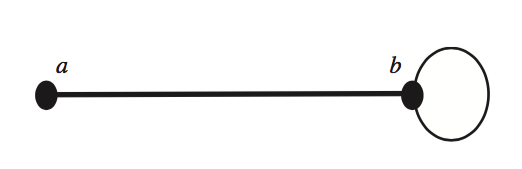
\includegraphics[width = 2.0in]{CMT2.png}
         \caption{\small{An example of a graph.}}
 \end{figure}

{\color{red}(Definitions Jasmine and I found but need a credible source for- currently looking for a textbook)}


\begin{definition}[Combinatorial Expression]
    A combinatorial expression is an expression with arithmetic operators as some terms
\end{definition}
    The Fibonacci and Lucas numbers are examples of this concept.

\begin{definition}[Power Sum] 
    A power sum is a sum of the $p^{th}$ powers on a set of $n$ variables
\end{definition}

\section{Graph Theory}
Graph Theory generalizes graphs and gives different theorems and concepts that can be used throughout our research.  Understanding different parts of the graph, what they mean for the research and how we can utilize them accordingly. In addition, we will use the definitions, theorems, and proofs from Linear Algebra to help explain the Graph Theory used in the next chapter.  

\cite{Graph_Theory}
\subsection{Graph Theory Definitions} %source: http://www.maths.ed.ac.uk/~aar/papers/wilsongraph.pdf
\begin{definition}[Graph]
    A graph is a physical representation of vertices (nodes), edges, and loops.
\end{definition}

\begin{definition}[Vertex]
    The vertex is the point on the graph.  It is also known as a node.  
\end{definition}

\begin{definition}[Edge]
    An edge is a path between two vertices.  
\end{definition}

\begin{figure}[h]
         \centering
         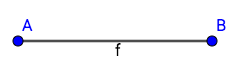
\includegraphics[width = 2.0in]{vertices.png}
         \caption{\small{$A$ and $B$ represent vertices. $f$ represents an edge.}}
 \end{figure}
Figure 2.2 demonstrate vertices and an edge.  The vertices both have degree 1.  
% source http://www.maths.ed.ac.uk/~aar/papers/wilsongraph.pdf
\begin{definition}[Degree]
    The degree of a vertex, $v$, is the number of edges incident with $v$, and is written deg(v). We can think of it as a number of roads at an intersection.\\
\end{definition}

\begin{figure}[h]
         \centering
         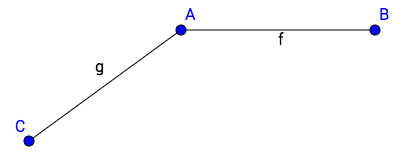
\includegraphics[width = 2.0in]{degree.png}
         \caption{\small{$A$ has a degree of 2 and $B$ and $C$ have a degree of one.}}
 \end{figure}
\par As seen in figure 2.3, the degree of each vertex is different.  A has a degree of 2 because it is connected to edges $f$ and $g$. 

\begin{definition}[Loop]
    A loop is an edge starting and ending at the same vertex.  
\end{definition}

A loop allows a vertex to have a closed walk of length one.

\begin{definition}[Walk]
    A walk is the path between one vertex to another vertex.  
\end{definition}

A walk is restricted to go from one node to another node.  If it does not make it from one node to another it is not considered a walk.
\begin{definition}[Path]
  A path is a walk in which no vertex appears more than once.  
\end{definition}

\begin{definition}[Cycle]
  A cycle is a walk begins at a particular vertex and ends that the same vertex.
\end{definition}
\todo{add definition of connected}
\begin{definition}[Closed Walk]
A closed walk is a path that begins at one particular vertex and ends at the same vertex. $(v_i$ to $v_i)$.
\end{definition}
Here is an example of a loop.
%\begin{figure}[h]
\begin{exmp}
Here are words
         \begin{center}
         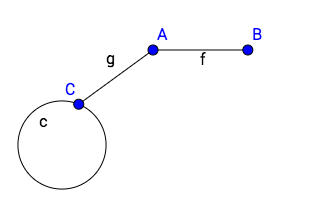
\includegraphics[width = 2.0in]{loops.png}
         \end{center}
\end{exmp}
        %\caption{\small{Vertex C contains a loop}}
 %\end{figure}
 % source: http://www.maths.ed.ac.uk/~aar/papers/wilsongraph.pdf
 \begin{definition}[Adjacency matrix]
   If $G$ is a graph with vertices ${1,2,\dots n}$ its adjacency matrix $A$ is the $n \times n$ matrix whose $ij$th entry is the number of edges joining vertex $i$ and vertex $j$. 
 \end{definition}

 \begin{exmp}
   Let us look at the figure below and determine its adjacency matrix.
 \end{exmp}

\begin{figure}[h]
         \centering
         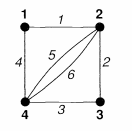
\includegraphics[width = 2.0in]{GTtbAM.png}
 \end{figure}
 \[ A =
 \begin{bmatrix}
   0  &  1  &  0  &  1 \\
   1  &  0  &  1  &  2 \\
   0  &  1  &  0  &  1 \\
   1  &  2  &  1  &  0
 \end{bmatrix}\] Therefore, we can see that in the $a_{11}$ entry we are looking at vertex 1 moving along an edge to get back to vertex 1.  There is no such vertex therefore the entry is 0. Notice the diagonals are 0. This is because those entries represent the walk from a vertex back to itself. This does not exist so all those entries are 0. 
 \par As defined earlier, the trace is the sum of the diagonals in the matrix. If we add these entries up, we also know how many closed walks there are. Thus for a closed walk of length 1, there are no closed walks.

In the next chapter there will be examples to demonstrate these concepts. The three subjects will be linked together to demonstrate the research and how each subject is important.
